
% v2-acmsmall-sample.tex, dated March 6 2012
% This is a sample file for ACM small trim journals
%
% Compilation using 'acmsmall.cls' - version 1.3 (March 2012), Aptara Inc.
% (c) 2010 Association for Computing Machinery (ACM)
%
% Questions/Suggestions/Feedback should be addressed to => "acmtexsupport@aptaracorp.com".
% Users can also go through the FAQs available on the journal's submission webpage.
%
% Steps to compile: latex, bibtex, latex latex
%
% For tracking purposes => this is v1.3 - March 2012
\documentclass[prodmode,acmtecs]{acmsmall} % Aptara syntax
\usepackage[spanish,polish]{babel}
\usepackage[T1]{fontenc}
\usepackage{fancyvrb}
\usepackage{graphicx,hyperref}
\newcommand\cutout[1]{}


\usepackage[table]{xcolor}
\usepackage[utf8]{inputenc}
\usepackage[parfill]{parskip}
\usepackage{tabulary}
\PassOptionsToPackage{hyphens}{url}
\usepackage{hyperref}    
\usepackage[capitalize]{cleveref}


% Metadata Information
% !!! TODO: SET THESE VALUES !!!
\acmVolume{0}
\acmNumber{0}
\acmArticle{CFP}
\acmYear{0}
\acmMonth{0}

\newcounter{colstart}
\setcounter{page}{4}

\RecustomVerbatimCommand{\VerbatimInput}{VerbatimInput}%
{
%fontsize=\footnotesize,
fontfamily=\rmdefault
}


\newcommand{\UnderscoreCommands}{%\do\verbatiminput%
\do\citeNP \do\citeA \do\citeANP \do\citeN \do\shortcite%
\do\shortciteNP \do\shortciteA \do\shortciteANP \do\shortciteN%
\do\citeyear \do\citeyearNP%
}

\usepackage[strings]{underscore}



% Document starts
\begin{document}


\setcounter{colstart}{\thepage}

\acmArticle{CFP}
\title{\huge\sc SIGLOG Monthly 225}
\author{DAVID PURSER\affil{University of Warsaw, Poland}
\vspace*{-2.6cm}\begin{flushright}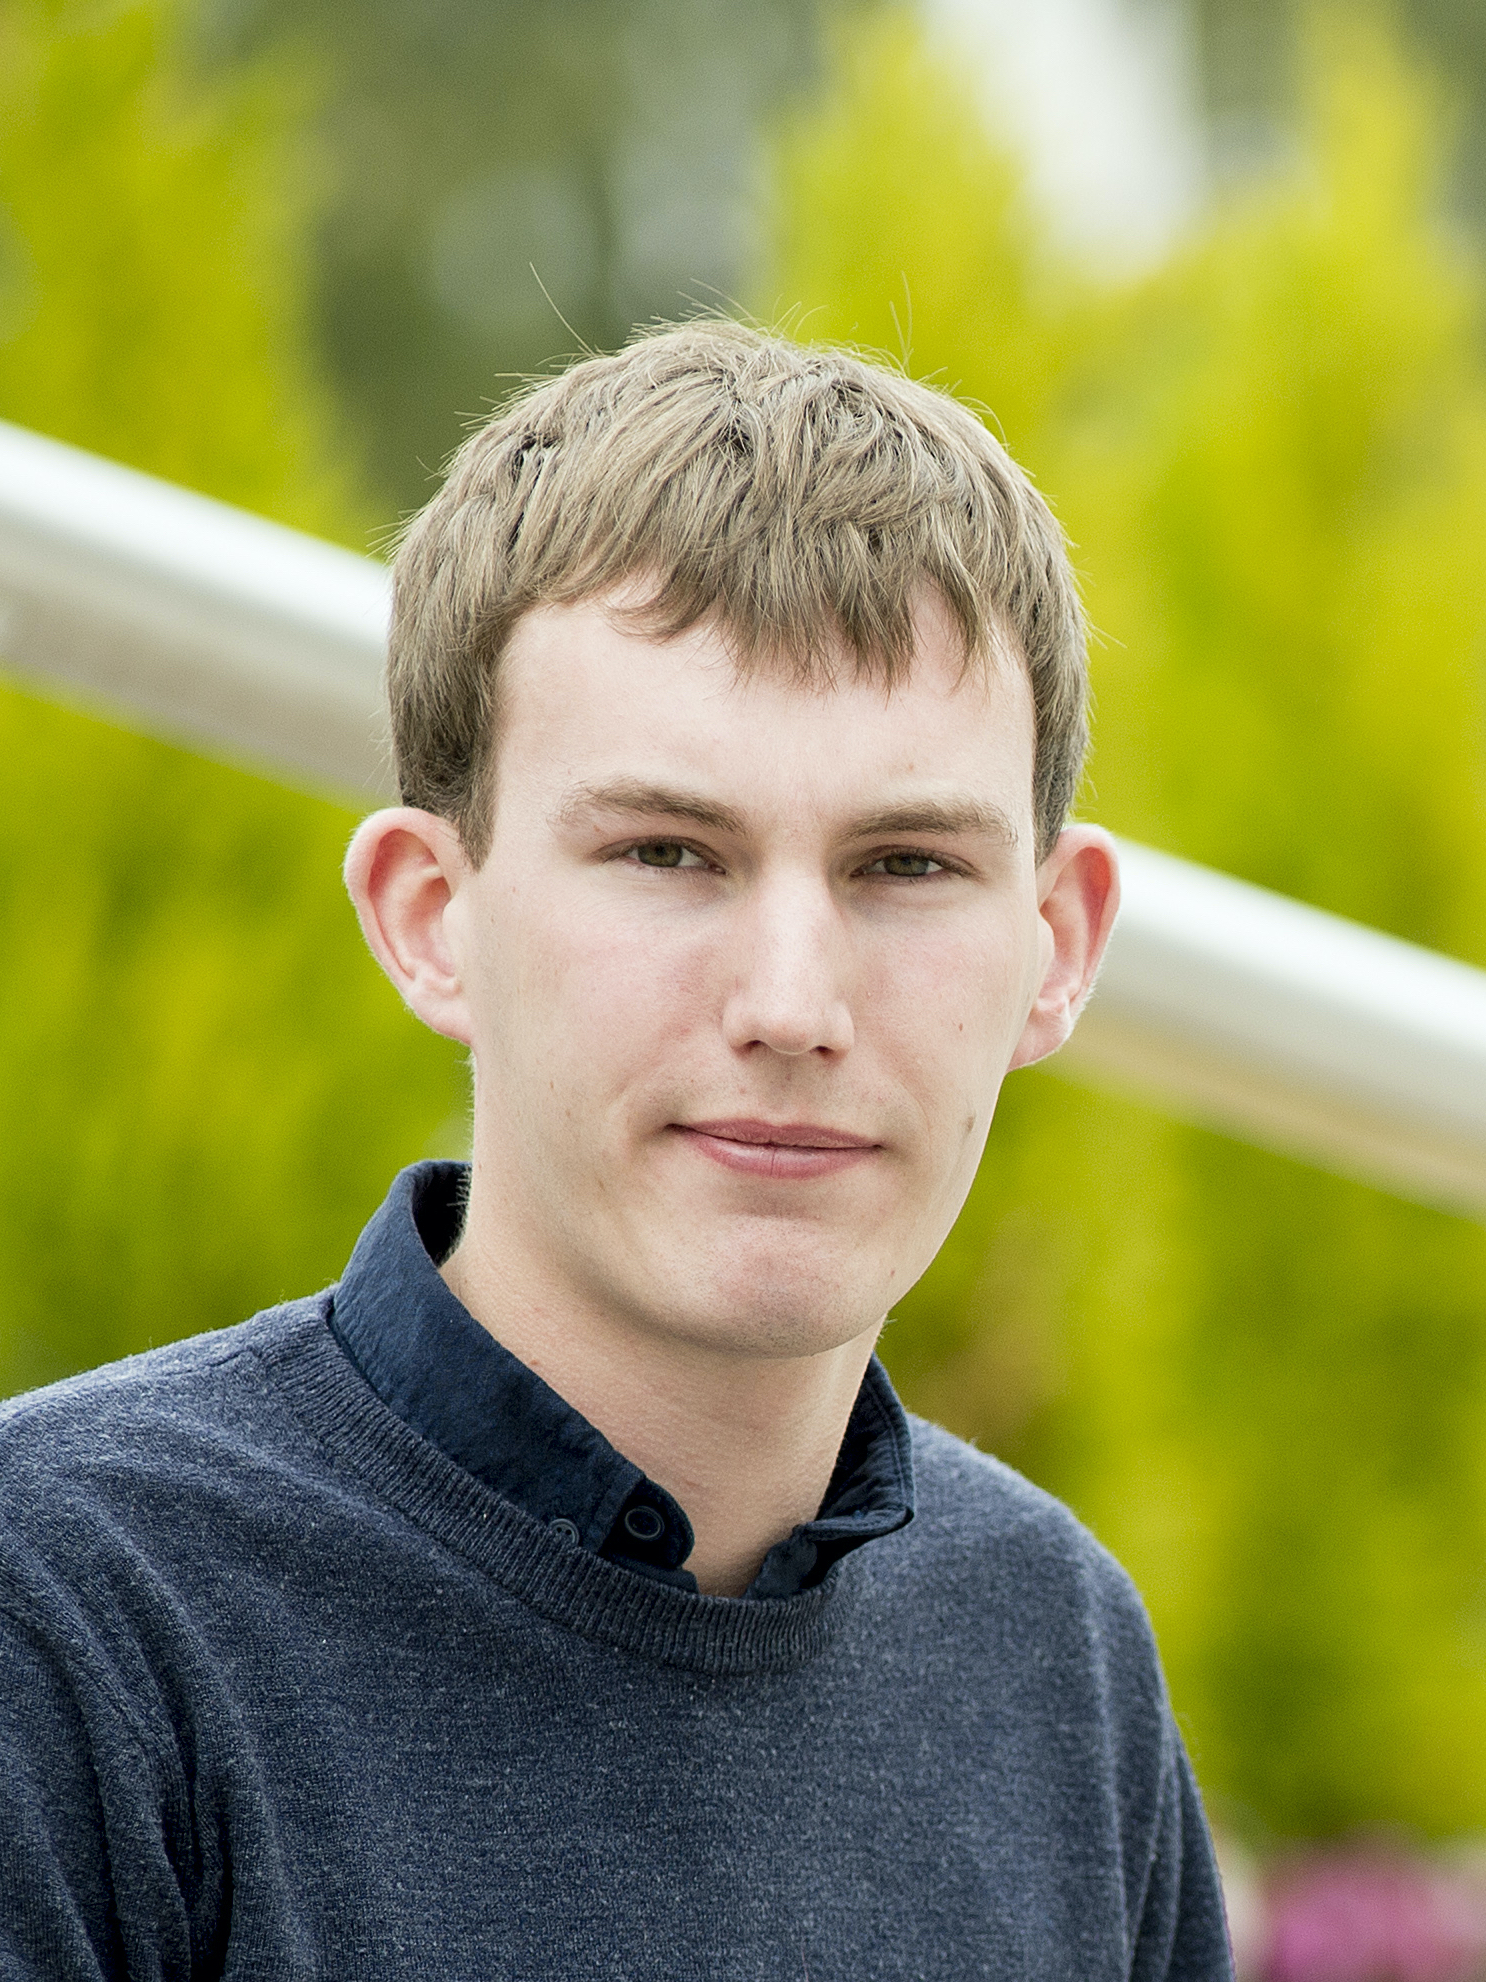
\includegraphics[width=30mm]{dp}\end{flushright}
}

\maketitlee

\href{https://lics.siglog.org/newsletters/}{Past Issues}
 - 
\href{https://lics.siglog.org/newsletters/inst.html}{How to submit an announcement}
\section{Table of Content}\begin{itemize}\item DEADLINES (\cref{deadlines}) 
 
\item CALLS 
 
\begin{itemize}\item SAS 2022 (CALL FOR PAPERS) (\cref{SAS2022})
\item CiE 2022 (CALL FOR INFORMAL PRESENTATIONS) (\cref{CiE2022})
\item ICALP 2022 (CALL FOR PARTICIPATION) (\cref{ICALP2022})
\item NFM 2022 (CALL FOR PARTICIPATION) (\cref{NFM2022})
\item PERR2022 (CALL FOR PAPERS/PRESENTATIONS) (\cref{PERR2022})
\item LogTeach-22 (CALL FOR CONTRIBUTIONS ) (\cref{LogTeach22})
\item ESSLLI 2022 (CALL FOR PARTICIPATION) (\cref{ESSLLI2022})
\end{itemize} 
\end{itemize}\section{Deadlines}\label{deadlines}\rowcolors{1}{white}{gray!25}\begin{tabulary}{\linewidth}{LL}ATVA 2022:  & May 01, 2022 (Abstract, extended), May 08, 2022 (Paper, extended) \\
MOVEP2022:  & May 01, 2022 (Student Abstract), Apr 30, 2022 (Early registration deadline) \\
IWC 2022:  & May 02, 2022 (Paper) \\
FORMATS 2022:  & May 04, 2022 (Abstract, extended), May 06, 2022 (Paper, extended) \\
SAS 2022:  & May 04, 2022 (Full paper), May 12, 2022 (Full paper updates until), May 18, 2022 (Artifact) \\
Runtime Verification 2022:  & May 05, 2022 (Paper) \\
ASL 2022:  & May 10, 2022 (Papers), May 10, 2022 (Papers due) \\
CiE 2022:  & May 10, 2022 (Abstracts of informal presentations) \\
NSV 2022:  & May 10, 2022 (Paper) \\
ICALP 2022:  & May 11, 2022 (Early Registration) \\
LAMAS\&SR 2022:  & May 23, 2022 (Paper) \\
PERR2022:  & May 28, 2022 (Submission Deadline) \\
PODS 2023:  & May 30, 2022 (First cycle abstract), Jun 06, 2022 (Full paper), Nov 28, 2022 (Second cycle abstract), Dec 05, 2022 (Full paper) \\
LogTeach-22:  & May 30, 2022 (Deadline for  of contributions) \\
ESSLLI 2022:  & May 31, 2022 (Early registration deadline) \\
FSCD 2024:  & Jun 27, 2022 (Deadline for proposals) \\
ACKERMANN AWARD 2022:  & Jul 01, 2022 (Deadline for nomination) \\
Datalog 2.0 2022:  & Jul 01, 2022 (Paper registration), Jul 08, 2022 (Paper) \\
\end{tabulary}
\section{SAS 2022: 29th Static Analysis Symposium}\label{SAS2022}  Auckland, New Zealand, December 5th-7th, 2022\\ 
  co-located with SPLASH\\ 
  \href{https://2022.splashcon.org/home/sas-2022}{https://2022.splashcon.org/home/sas-2022}\\ 
CALL FOR PAPERS 

\begin{itemize}\item  CONFERENCE 
 
  The 28th Static Analysis Symposium, SAS 2022, will be co-located with SPLASH 2022 in Auckland, New Zealand. 
 
  Static Analysis is widely recognized as a fundamental tool for program verification, bug detection, compiler optimization, program understanding, and software maintenance. The series of Static Analysis Symposia has served as the primary venue for the presentation of theoretical, practical, and application advances in the area. 
 
\item  IMPORTANT DATES 
 
\rowcolors{1}{white}{gray!25}\begin{tabulary}{\linewidth}{LL}Full paper submission:  & May 04, 2022 \\
Full paper updates until:  & May 12, 2022 \\
Artifact submission:  & May 18, 2022 \\
Author response period:  & Jun 27-30, 2022 \\
Notification:  & Jul 15, 2022 \\
Final version due:  & Sep 16, 2022 \\
Conference:  & Dec 5-7, 2022 \\
\end{tabulary}
 
\item  PAPER SUBMISSION 
 
  All paper submissions will be judged on the basis of significance, relevance, correctness, originality, and clarity. Submission link: \href{https://easychair.org/conferences/?conf=sas2022}{https://easychair.org/conferences/?conf=sas2022} We welcome regular papers as well as papers focusing on any of the following: 
 
\begin{itemize}\item   Experience with static analysis tools, Industrial Reports, and Case Studies
\item   Tool papers
\item   Brief announcements of work in progress
\item   Well-motivated discussion of new questions or new areas. We do not impose a page limit for submitted papers but we encourage brevity as reviewers have a limited time that they can spend on each paper. With the exception of experience papers, all other papers will follow a lightweight double-blind reviewing process.
\end{itemize} 
\item  RADHIA COUSOT AWARD 
 
  The program committee will select an accepted regular paper for the Radhia Cousot Young Researcher Best Paper Award in memory of Radhia Cousot and her fundamental contributions to static analysis, as well as being one of the main promoters and organizers of the SAS series of conferences. 
 
\item  ARTIFACTS 
 
  As in previous years, we encourage authors to submit a virtual machine image containing any artifacts and evaluations presented in the paper. Artifact submission is optional. Artifact evaluation will be concurrent with paper review. 
 
\end{itemize}\section{CiE 2022: Computability in Europe 2022 Revolutions and revelations in computability}\label{CiE2022}  CiE 2022 is planned as an on-site conference with online elements \\ 
  Swansea, Wales, United Kingdom\\ 
  July 11-15, 2022\\ 
  \href{https://cs.swansea.ac.uk/cie2022/}{https://cs.swansea.ac.uk/cie2022/}\\ 
CALL FOR INFORMAL PRESENTATIONS 

\begin{itemize}\item  Continuing the tradition of past CiE conferences, we invite researchers to present informal presentations of their recent work. A proposal for an informal presentation must be submitted via EasyChair (\href{https://easychair.org/conferences}{https://easychair.org/conferences} /?conf=cie2022), using the LNCS style file, and be 1 page long; a brief description of the results suffices and an abstract is not required. Informal presentations will not be published in the LNCS conference proceedings. Results presented as informal presentations at CiE 2022 may appear or may have appeared in other conferences with formal proceedings and/or in journals. The deadline for the submission of abstracts for informal presentations is May 10, 2022. The notifications of acceptance for informal presentations will be sent a few days after submission. 
 
\end{itemize}\section{ICALP 2022: International Colloquium on Automata, Languages, and Programming}\label{ICALP2022}  Paris, France, and online on 4-8 July 2022\\ 
  \href{https://icalp2022.irif.fr/}{https://icalp2022.irif.fr/}\\ 
CALL FOR PARTICIPATION 

\begin{itemize}\item  The 2022 edition has the following special features: - The conference is hybrid. - This will be the 50th birthday of the conference and some special events are planned. - The ICALP Extended Stay Support Scheme (IESSS) is here for helping the organisation of collaborations around the conference. 
 
  ICALP is the main conference and annual meeting of the European Association for Theoretical Computer Science (EATCS). As usual, ICALP will be preceded by a series of workshops, which will take place on July 4. 
 
  The 2022 edition will be also the occasion to celebrate the 50th anniversary of both EATCS and the first ICALP, which was first held in 1972 in Rocquencourt, in the Paris area. 
 
\item  IMPORTANT DATES AND INFORMATION  
 
\rowcolors{1}{white}{gray!25}\begin{tabulary}{\linewidth}{LL}Early Registration:  & May 11, 2022 \\
Conference:  & Jul 4-8, 2022 \\
Workshops:  & Jul 04, 2022 \\
\end{tabulary}
 
\item  REGISTRATION  
 
  For registration, follow this link: \href{https://icalp2022.irif.fr/?page_id=50}{https://icalp2022.irif.fr/?page\_id=50} 
 
\item  EXTENDED STAY SUPPORT SCHEME (IESS)  
 
  For its 49th edition, the ICALP conference offers to its attendees an Extended Stay Support Scheme (IESSS) aiming at enhancing scientific collaborations and diminishing the carbon footprint of scientific research activities. ICALP 2022 attendees are encouraged to combine their visit to Paris with collaborations with local researchers. 
 
  This support scheme is primarily intended for participants travelling long distances and must be combined with an attendance to ICALP. Upon acceptation, research institutes involved in this mechanism will cover standard expenses (accommodation and traveling fees, plane excluded) and will provide material support for research activities. 
 
  See \href{https://icalp2022.irif.fr/?page_id=50}{https://icalp2022.irif.fr/?page\_id=50} for more information. 
 
\item  INVITED SPEAKERS  
 
\begin{itemize}\item  Albert Atserias, Universitat Politècnica de Catalunya
\item  Constantinos Daskalakis, MIT 
\item  Leslie Ann Goldberg, Oxford University 
\item  Madhu Sudan, Harvard 
\item  Stéphan Thomassé, ENS Lyon 
\item  Santosh Vempala, Georgia Tech
\end{itemize} 
\item  AWARDS  
 
  During the conference, the following awards will be given: 
 
\begin{itemize}\item  the EATCS award (\href{https://eatcs.org/index.php/eatcs-award}{https://eatcs.org/index.php/eatcs-award}),
\item  the Gödel prize (\href{https://eatcs.org/index.php/goedel-prize}{https://eatcs.org/index.php/goedel-prize}),
\item  the Presburger award (\href{https://eatcs.org/index.php/presburger}{https://eatcs.org/index.php/presburger}),
\item  the EATCS distinguished dissertation award (\href{https://eatcs.org/index.php/dissertation-award}{https://eatcs.org/index.php/dissertation-award}),
\item  the best papers for Track A and track B,
\item  the best student papers for Track A and track B.
\end{itemize} 
\item  ACCEPTED PAPERS  
 
  See \href{https://icalp2022.irif.fr/?page_id=85}{https://icalp2022.irif.fr/?page\_id=85}  
 
\item  WORKSHOPS  
 
  See \href{https://icalp2022.irif.fr/?page_id=46}{https://icalp2022.irif.fr/?page\_id=46} for more information. 
 
\begin{itemize}\item  Parameterized Approximation Algorithms Workshop 
\item  Combinatorial Reconfiguration 
\item  Recent Advances on Total Search Problems 
\item  Algorithmic Aspects of Temporal Graphs V 
\item  Trends in Arithmetic Theories 
\item  Structure Meets Power 2022 
\item  Straight-Line Programs, Word Equations and their Interplay 
\item  Graph Width Parameters: from Structure to Algorithms
\end{itemize} 
\end{itemize}\section{NFM 2022: 14th NASA Formal Methods Symposium }\label{NFM2022}  NFM 2022 is organized by Jet Propulsion Laboratory, USA \\ 
  May 24-27, 2022\\ 
  Pasadena, California, USA (MIXED PHYSICAL + VIRTUAL SYMPOSIUM)\\ 
  \href{https://nfm2022.caltech.edu}{https://nfm2022.caltech.edu}\\ 
  Free Registration: \href{https://nfm2022.caltech.edu/register}{https://nfm2022.caltech.edu/register}\\ 
CALL FOR PARTICIPATION 

\begin{itemize}\item  After two years of virtual NFM symposia, we are returning to arranging a physical event. However, virtual participation is supported for those who prefer this option. 
 
\item  THEME OF THE SYMPOSIUM 
 
  The complexity of mission-critical and safety-critical systems at NASA and in the aerospace industry requires advanced techniques to address their specification, design, verification, validation, and certification. The NASA Formal Methods Symposium (NFM) is a forum to foster collaboration between theoreticians and practitioners from NASA, academia, and industry working on formal methods to develop and apply such techniques.  
 
  The NASA Formal Methods Symposium is an annual event organized by the NASA Formal Methods Research Group, composed of researchers spanning six NASA centers.  
 
\item  REGISTRATION 
 
  There is no registration fee charged to participants. Register here: \href{https://nfm2022.caltech.edu/register}{https://nfm2022.caltech.edu/register}  
 
\item  KEYNOTE SPEAKERS 
 
\begin{itemize}\item  Dines Bjørner (Technical University of Denmark, Denmark
\item  Steve Chien (Jet Propulsion Laboratory, USA
\item  Daniel Jackson (MIT CSAIL, USA
\item  Julia Lawall (Inria-Paris, France
\item  Sriram Sankaranarayanan (University of Colorado Boulder, USA
\item  Alex Summers (University of British Columbia, Canada
\item  Emina Torlak (University of Washington, USA)
\end{itemize} 
\item  TUTORIALS 
 
\begin{itemize}\item  Edwin Brady (University of St. Andrews, UK)
\item  Ankush Desai (Amazon Web Services, USA)
\item  Anastasia Mavridou (KBR Inc/NASA Ames Research Center, USA)
\item  Leonardo de Moura (Microsoft Research, USA)
\item  Sebastian Ullrich (Karlsruhe Institute of Technology, Germany)
\end{itemize} 
\end{itemize}\section{PERR2022: 5th Workshop on Program Equivalence and Relational Reasoning }\label{PERR2022}  August 11, 2022 at Technion, Haifa, Israel associated with CAV 2022 at FLOC 2022 \\ 
  \href{https://perr-workshop.github.io/2022}{https://perr-workshop.github.io/2022}\\ 
  Submission Deadline: Friday, 28 May, 2022 (AoE)\\ 
  Submit at: \href{https://easychair.org/conferences/?conf=perr2022}{https://easychair.org/conferences/?conf=perr2022}\\ 
CALL FOR PAPERS/PRESENTATIONS 

\begin{itemize}\item  PERR is an annual international workshop dedicated to the formal verification of program equivalence and related relational problems. It is the 5th in a series of meetings that bring together researchers from different areas interested in equivalence and related questions. PERR 2022 will be a workshop at FLOC 2022, and a satellite event to CAV 2022. 
 
  Program equivalence is arguably one of the most interesting and at the same time important problems in formal verification. It is a cross-cutting topic that has attracted the interest of several research communities: the field of denotational (game) semantics, deductive software verification, bounded model checking, specification inference, software evolution and regression testing, etc. 
 
  The goal of the workshop is to bring researchers of the different fields in touch and to stipulate an exchange of ideas leading to forging a community working on PERR. It welcomes contributions from the topics mentioned above but is also open to new questions regarding program equivalence. This includes related research areas of relational reasoning like program refinement or the verification of hyperproperties, in particular of secure information flow. 
 
\begin{itemize}\item  regression verification 
\item  program equivalence 
\item  equivalence of higher order programs 
\item  product programs, relational calculi 
\item  verification of hyperproperties 
\item  program refinement, refinement calculus 
\item  specification of differences between programs 
\item  inferring semantic differences between programs 
\item  transformation validation 
\item  correct compiler transformations 
\item  automata bisimulation 
\item  code equivalence checking in teaching and marking
\end{itemize} 
  This is an informal workshop that welcomes work in progress, overviews of more extensive work, programmatic or position papers and tool presentations. 
 
\item  SUBMISSION GUIDELINES 
 
  Please submit an abstract (this can be in the form of 1-2 pages of text, or a paper of no more than 15 pages in LNCS format) of your proposed talk on the EasyChair submission page below. Submissions will be reviewed by at least 2 PC members and feedback will be provided. 
 
 \href{https://easychair.org/conferences/?conf=perr2022}{https://easychair.org/conferences/?conf=perr2022} 
 
  The workshop will have informal proceedings, posted on the webpage, and speakers will be asked to consider submitting papers towards a post-proceedings volume (to be published e.g. as a technical report). 
 
\item  IMPORTANT DATES (AoE)  
 
\rowcolors{1}{white}{gray!25}\begin{tabulary}{\linewidth}{LL}Submission Deadline:  & May 28, 2022 \\
Notification:  & Jul 01, 2022 \\
Workshop:  & Aug 11, 2022 \\
\end{tabulary}
 
\end{itemize}\section{LogTeach-22: Why and how to teach Logic for CS undergraduates? }\label{LogTeach22}  \href{https://www.cs.technion.ac.il/~janos/LogTeach-22/}{https://www.cs.technion.ac.il/~janos/LogTeach-22/} \\ 
  LICS 2022 Workshop (July 31 and August 1, 2022, Haifa)\\ 
  FLOC is planned to be a conference with physical presence (possibly hybrid) in Haifa.\\ 
  \href{https://easychair.org/cfp/LogTeach-22}{https://easychair.org/cfp/LogTeach-22}\\ 
CALL FOR CONTRIBUTIONS  

\begin{itemize}\item  SCIENTIFIC JUSTIFICATION  
 
  Logic is one of the pillars of the foundation of Computer Science, together with Algorithmic Mathematics, Information Theory, and Electronics. Consequently various versions of Logic courses used to be part of the undergraduate syllabus of Computer Science. However, as witnessed by the variety of conferences related to Logic present at the FLoC event, the emphasis has moved from the foundation to applications of Logic in Computer Science. Each of these conferences deal with topics suitable for advanced undergraduate and graduate courses, which require some Logic based prerequisite. On the other hand, Logic courses in the undergraduate syllabus have been forced to make place for courses deemed more suitable for the education of future specialists and practitioners working in IT. Many of the top Universities worldwide have dropped foundational Logic courses for undergraduates for more practical oriented courses, turning undergraduate CS programs into programs more suitable for what used to be vocational colleges and professional schools. 
 
  Time has come to critically reflect upon and reevaluate the role of Logic in the undergraduate syllabus. It seems clear that the classical Logic in CS courses have no place there anymore. They seem to teach and emphasize the wrong narrative of logic as taught by tradition. However, it seems also clear that eliminating Logic courses all together is counter productive. The purpose of the workshop is the prepare a proposal for a logic course Logic-2020 which is useful and acceptable for University undergraduates in CS, and which can serve as a prerequisite for the many diverse branches of applied logic. 
 
  Georg Kreisel: ``Logic may be not very useful, if you know it, but very harmful, if you ignore it''  
 
\item  INVITED SPEAKERS (updated) 
 
\begin{itemize}\item  Moshe Vardi (Rice University, Houston TA, USA) 
\item  Matthias Baaz (Technical University, Vienna, Austria) 
\item  Reinhold Kahle (Universität Tübingen, Tübingen, Germany) 
\item  Arnon Avron (TA University, Tel Aviv, Israel) 
\item  Martin Davis (Courant Institute, New York, USA) 
\item  Thomas Zeume (Ruhr Universität Bochum, Germany)
\end{itemize} 
  To be completed 
 
\item  CONTRIBUTED TALKS 
 
  We invite contributed talks, which can be 15 minute or 30 minutes (including discussion). This will serve as the basis for the planned panel discussion. Contributers should submit a pdf-file of an abstract or summary of atmost 3 pages at \href{https://easychair.org/cfp/LogTeach-22}{https://easychair.org/cfp/LogTeach-22} till 30. May, 2022. Full papers may be additionally submitted only as a second submission besides the 3 page version. 
 
\item  ORGANISATION  
 
  The purpose of the workshop is to prepare a joint position paper to be published possibly in the Communications of ACM, or a similar prominent place, with recommendations for the future of teaching Logic for undergraduate CS-students. We plan to have presentations of position papers (30 minutes, including discussion) and invited lectures (60 minutes including discussion), followed by a two hour panel discussion. 
 
\item  DATES    
 
\rowcolors{1}{white}{gray!25}\begin{tabulary}{\linewidth}{LL}Deadline for submission of contributions:  & May 30, 2022 \\
Notification of acceptance:  & Jun 20, 2022 \\
\end{tabulary}
 
  Submission link: \href{https://easychair.org/conferences/?conf=logteach22}{https://easychair.org/conferences/?conf=logteach22}  
 
\end{itemize}\section{ESSLLI 2022: European Summer School in Logic, Language and Information}\label{ESSLLI2022}  Galway, Ireland \\ 
CALL FOR PARTICIPATION 

\begin{itemize}\item   Registration is now open for the 33rd European Summer School in Logic, Language and Information (ESSLLI), taking place from 8-19 August, 2022 at the National University of Ireland Galway: \href{https://2022.esslli.eu/}{https://2022.esslli.eu/} 
 
\item  OVERVIEW 
 
  The European Summer School in Logic, Language and Information (ESSLLI) is a yearly recurring event, organised under the auspices of the Association for Logic, Language and Information (FoLLI), and has been running since 1989. The ESSLLI Summer School provides an interdisciplinary setting in which courses and workshops are offered in logic, linguistics and computer science, also from wider scientific, historical, and philosophical perspectives. 
 
  ESSLLI attracts around 400 participants from all parts of Europe, as well as from North and Latin America, and Asia. The ESSLLI has become the main meeting place for young researchers and students in logic, linguistics and computer science to discuss current research and to share knowledge. The event is unique in its interdisciplinary set-up, with no equivalents in Europe. 
 
\item  PROGRAMME 
 
  The ESSLLI Summer School offers an exciting two-week programme, consisting of the following:  
 
\begin{itemize}\item  Workshops in logic, linguistics and computer science 
\item  Courses, foundational, introductory and advanced, in three areas: Language and Computation, Logic and Computation, and Logic and Language 
\item  Student session 
\item  Evening lectures 
\item  Social activities
\end{itemize} 
\item  REGISTRATION 
 
  Registration for attendees, course lecturers, student session and workshop organisers and speakers is now open. \href{https://2022.esslli.eu/registration.html}{https://2022.esslli.eu/registration.html}.  
 
Early registration deadline: May 31, 2022 
 
\end{itemize}


To the \href{http://siglog.org/}{SIGLOG} or \href{https://lics.siglog.org}{LICS} website\end{document}